\documentclass[twoside]{article}

\usepackage{aistats2020}
% If your paper is accepted, change the options for the package
% aistats2020 as follows:
%
% \usepackage[accepted]{aistats2020}
%
% This option will print headings for the title of your paper and
% headings for the authors names, plus a copyright note at the end of
% the first column of the first page.

% If you set papersize explicitly, activate the following three lines:
%\special{papersize = 8.5in, 11in}
%\setlength{\pdfpageheight}{11in}
%\setlength{\pdfpagewidth}{8.5in}

% If you use natbib package, activate the following three lines:
\usepackage[round]{natbib}
\renewcommand{\bibname}{References}
\renewcommand{\bibsection}{\subsubsection*{\bibname}}

\usepackage[draft]{hyperref}       % hyperlinks
\usepackage{url}            % simple URL typesetting
\usepackage{booktabs}       % professional-quality tables
\usepackage{amsfonts}       % blackboard math symbols
\usepackage{nicefrac}       % compact symbols for 1/2, etc.
\usepackage{microtype}      % microtypography
\usepackage{amsmath}
\usepackage{graphicx}
\usepackage{setspace}
\usepackage{caption}
\usepackage{subcaption}

\usepackage{enumitem}       % customize list indentation

\usepackage{algorithm}
\usepackage{algorithmicx}
\usepackage[noend]{algpseudocode}
\renewcommand{\algorithmicrequire}{\textbf{Input:}}
\renewcommand{\algorithmicensure}{\textbf{Output:}}

\algnewcommand\algorithmicassert{\texttt{assert}}
\algnewcommand\Assert[1]{\State{} \algorithmicassert(#1)}

\algnewcommand\algorithmicswitch{\textbf{switch}}
\algnewcommand\algorithmiccase{\textbf{case}}
\algnewcommand\algorithmicdefault{\textbf{default}}
\algdef{SE}[SWITCH]{Switch}{EndSwitch}[1]{\algorithmicswitch\ #1\ \algorithmicdo}{\algorithmicend\ \algorithmicswitch}
\algdef{SE}[CASE]{Case}{EndCase}[1]{\algorithmiccase\ #1}{\algorithmicend\ \algorithmiccase}
\algdef{SE}[DEFAULT]{Default}{EndDefault}[1]{\algorithmicdefault\ #1}{\algorithmicend\ \algorithmicdefault}
\algtext*{EndSwitch}
\algtext*{EndCase}
\algtext*{EndDefault}

\algnewcommand\algorithmicmatch{\textbf{match}}
\algdef{SE}[MATCH]{Match}{EndMatch}[1]{\algorithmicmatch\ #1}{\algorithmicend\ \algorithmicmatch}
\algtext*{EndMatch}

\algnewcommand\algorithmictry{\textbf{try}}
\algnewcommand\algorithmiccatch{\textbf{catch}}
\algblockdefx[Try]{Try}{EndTry}{\algorithmictry}{\algorithmicend\ \algorithmictry}
\algtext*{EndTry}
\algcblockdefx[Catch]{Try}{Catch}{EndTry}[1]{\algorithmiccatch\ #1}{\algorithmicend\ \algorithmictry}%
\algtext*{EndTry}
\MakeRobust{\Call}

\algdef{SE}[QUERY]{Query}{EndQuery}%
   [2]{\textbf{query}\ \textproc{#1}\ifthenelse{\equal{#2}{}}{}{(#2)}}%
   {\algorithmicend\ \algorithmicquery}%
\algtext*{EndQuery}

\def\@algocf@capt@ruled{under}

\usepackage{hyperref}

% !TEX root =  nips_dtfa.tex

%% OPTIONAL MACRO DEFINITIONS
% operators
\newcommand{\argmax}{\operatornamewithlimits{argmax}}
\newcommand{\argmin}{\operatornamewithlimits{argmin}}

% fractions, derivatives
\newcommand{\pdff}[2]{\frac{\partial #1}{\partial #2}}
\newcommand{\fdff}[2]{\frac{\delta #1}{\delta #2}}
\newcommand{\ifrac}[2]{#1 \:/\: #2}

% conditional probability 
\newcommand{\p}[2]{\ensuremath{p(#1 \mid #2)}}
\newcommand{\q}[2]{\ensuremath{q(#1 \mid #2)}}
\renewcommand{\d}[1]{\ensuremath{\!\!d#1 \:}}

% vectors
\renewcommand{\vec}[1]{\ensuremath{\boldsymbol{#1}}}
\renewcommand{\v}[1]{\vec{#1}}
\newcommand{\x}{\ensuremath{\v{x}}}
\newcommand{\y}{\ensuremath{\v{y}}}
\newcommand{\z}{\ensuremath{\v{z}}}
\newcommand{\h}{\ensuremath{\v{\eta}}}
\renewcommand{\u}{\ensuremath{u}}
\renewcommand{\q}{\ensuremath{\theta}}
\renewcommand{\l}{\ensuremath{\lambda}}
\renewcommand{\t}{\ensuremath{\tau}}
\newcommand{\f}{\ensuremath{\phi}}

% misc symbols
\newcommand{\KL}[2]{\ensuremath{D_{\rm KL}\left(#1 \:\middle\vert\middle\vert\: #2\right)}}
\renewcommand{\L}{\ensuremath{\mathcal{L}}}
\renewcommand{\P}{\ensuremath{{\mathcal P}}}
\renewcommand{\S}{\ensuremath{\mathcal{S}}}
\renewcommand{\O}{\ensuremath{\mathcal{O}}}
\newcommand{\C}{\ensuremath{\mathcal{C}}}
\newcommand{\Q}{\ensuremath{\mathcal{Q}}}
\newcommand{\V}{\ensuremath{\mathcal{V}}}
\newcommand{\F}{\ensuremath{\mathcal{F}}}
\newcommand{\U}{\ensuremath{\mathcal{U}}}
\newcommand{\E}{\ensuremath{\mathcal{E}}}
\newcommand{\G}{\ensuremath{\mathcal{G}}}
\newcommand{\M}{\ensuremath{\mathcal{M}}}
\newcommand{\N}{\ensuremath{\mathcal{N}}}
\newcommand{\bs}{\backslash}
\newcommand{\td}{\tilde}

\newcommand{\indicator}[2]{\ensuremath{\mathbb{I}{[{#1}={#2}]}}}
\newcommand*{\dom}{\ensuremath{\mathrm{dom}}}

\newcommand{\norm}[1]{\left\lVert#1\right\rVert}

\newcommand{\scf}{\textsc{f}}
\newcommand{\scg}{\textsc{g}}
\newcommand{\scw}{\textsc{w}}
\newcommand{\scp}{\textsc{p}}
\newcommand{\scs}{\textsc{s}}
\newcommand{\scx}{\textsc{x}}

% hyperref makes hyperlinks in the resulting PDF.
% If your build breaks (sometimes temporarily if a hyperlink spans a page)
% please comment out the following usepackage line and replace
% \usepackage{icml2019} with \usepackage[nohyperref]{icml2019} above.

% If you use BibTeX in apalike style, activate the following line:
%\bibliographystyle{apalike}

\begin{document}

% Attempt to make hyperref and algorithmic work together better:
\renewcommand{\theHalgorithm}{\arabic{algorithm}}

% If your paper is accepted and the title of your paper is very long,
% the style will print as headings an error message. Use the following
% command to supply a shorter title of your paper so that it can be
% used as headings.
%
%\runningtitle{I use this title instead because the last one was very long}

% If your paper is accepted and the number of authors is large, the
% style will print as headings an error message. Use the following
% command to supply a shorter version of the authors names so that
% they can be used as headings (for example, use only the surnames)
%
%\runningauthor{Surname 1, Surname 2, Surname 3, ...., Surname n}

\twocolumn[
    \aistatstitle{Neural Topographic Factor Analysis for fMRI Data}
    
    % \aistatsauthor{ Eli Z.~Sennesh \And Zulqarnain Khan \And Jennifer Dy \And Ajay B. Satpute }
    % \aistatsauthor{ J. Benjamin Hutchinson \And Jan-Willem van de Meent }
    
    % \aistatsaddress{ Northeastern University }
]

\begin{abstract}
  Functional magnetic resonance imaging experiments produce gigabytes of high-dimensional spatio-temporal data for a small number of sampled participants and stimuli. Analyses of this data commonly average over all trials, ignoring variation among participants and stimuli. As a means of reasoning about this variation, we propose Neural Topographic Factor Analysis (NTFA), a deep generative model that parameterizes factors as functions of embeddings for participants and stimuli. We evaluate NTFA on a synthetically generated dataset, results from an in-house pilot study, and two publicly available datasets. We demonstrate that NTFA produces more accurate reconstructions with fewer parameters than related methods. Moreover, NTFA constitutes a first step towards reasoning about individual variation; learned embeddings uncover latent categories of stimuli, and partially separate latent groups of participants.  
\end{abstract}

\vspace{-1em}
\section{Introduction}
\vspace{-1em}

Analyzing neuroimaging studies is both a large data problem and a small data problem.  A single scanning run typically involves hundreds of full-brain scans that each contain tens of thousands of spatial locations (known as voxels). At the same time, neuroimaging studies tend to have limited statistical power. A typical study considers a cohort of 20-50 participants undergoing tens (or fewer) stimuli.  A largely unsolved challenge in this domain is to develop analysis methods that appropriately account for both the commonalities and variations among participants and stimulus effects, scale to tens of gigabytes of data, and reason about uncertainty to guard against overconfident predictions.

In this paper, we develop Neural Topographic Factor Analysis (NTFA)%\footnote{Source code submitted with paper and available on Github by request.}
, a family of models for analysis of spatio-temporal fMRI data that is suitable for reasoning about variations among participants and stimuli. NTFA extends Topographic Factor Analysis (TFA), an established method for fMRI analysis \citep{manning2014topographic}, with a deep generative prior. This prior defines a distribution over embeddings (i.e.~vectors of features) for each participant and stimulus, along with a conditional distribution over spatial and temporal factors, which is parameterized by a simple neural network. The result is a structured deep probabilistic model that can characterize variation among participants and stimuli, as well as interaction effects.

Our experiments compare NTFA to hierarchical topographic factor analysis (HTFA) \citep{manning2014hierarchical,manning2018probabilistic}, a closely related method that employs a hierarchical Gaussian prior in lieu of our structured deep probabilistic model. We evaluate a total of four datasets, including data from a previously unpublished pilot study by the authors:
\begin{itemize}[labelwidth=0.5em, 
                labelsep=0.5em, 
                leftmargin=1.0em,
                topsep=0em,
                label={\tiny\raisebox{0.7ex}{\textbullet}}]
\item As a basic validation of our model, we show that inference and learning recover the true group structure in a synthetic dataset that was simulated from generative model with clearly distinguishable clusters of participants and stimuli. 

\item We present results for a pilot study on the neural basis of fear, carried out by the authors. In this study, participants are shown video clips of spiders, looming heights, and threatening social situations. The clips vary in how much fear they evoked, both within each category and across individuals. The stimulus embeddings learned by NTFA, which are fully unsupervised, group according to actual stimulus categories, and participant embeddings correlate with behavioral measures.

\item Finally, we consider two publicly available datasets. In the first, participants listen to the narrative ``Pie Man'' \citep{simony2016dynamic}. In the second, participants with major depressive disorder and controls listen to audio stimuli and music \citep{10.1371/journal.pone.0156859}. We find that NTFA yields more accurate reconstructions than HTFA, while employing a smaller number of trainable parameters.
\end{itemize}

\begin{figure*}[!t]
    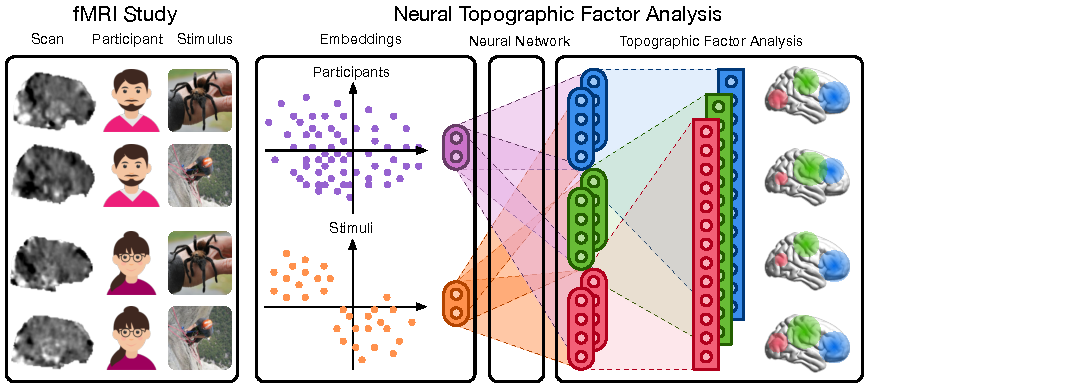
\includegraphics[width=\textwidth]{figures/neural-tfa-v5-cropped.pdf}
    \caption{\textbf{Overview of Neural Topographic Factor Analysis (NTFA)}: We extend topographic factor analysis (TFA) \citep{manning2014topographic,manning2014hierarchical} to decompose the fMRI signal into Gaussian factors (shown in red, green and blue in the figure) that correspond to spatially and temporally related brain activity across individuals. We represent participants (purple) and stimuli (orange) with embedding vectors. A decoder network then predicts the location, size, and mean response.}
    \label{fig:overview}
\end{figure*}

Based on these findings, we believe that NTFA represents a meaningful step towards developing models that are able to characterize individual variation in an unsupervised manner. Concretely, the contributions of this paper can be summarized as follows:

% \vspace{-0.75em}
\begin{itemize}[labelwidth=0.5em, 
                labelsep=0.5em, 
                leftmargin=1.0em,
                topsep=0em,
                label={\tiny\raisebox{0.7ex}{\textbullet}}]
    \item We develop NTFA (Section~\ref{sec:ntfa-basic}), a new model for analysis of fMRI data that infers embeddings for participants and stimuli that are shared across experiment trials. We perform inference using black-box variational methods that are implemented in Probabilistic Torch \citep{narayanaswamy2017learning}.
    \item We show that NTFA achieves a lower reconstuction loss with fewer trainable parameters than HTFA, which is representative of the state of the art.
    \item We demonstrate that embeddings, learned without supervision, correlate with experimental design variables and behavioral measures (Section~\ref{subsec:evaluation}). To our knowledge, NTFA is the first model able to characterize participants and stimuli in this way.
\end{itemize}
% \vspace{-0.75em}

Figure \ref{fig:overview} shows an overview of the proposed approach. Section \ref{sec:background} covers the related work in Factor Analysis for neuroimaging data, primarily HTFA which forms the basis for this work. Section \ref{sec:ntfa-basic} develops the NTFA model and Section \ref{sec:experiments} discusses experiments and results.

\vspace{-1em}
\section{Background}
\vspace{-1em}
\label{sec:background}

Factor analysis methods are widely used to reduce the dimensionality of neuroimaging data. These methods decompose the fMRI signal for a trial $Y \in \mathbb{R}^{T\text{x}V}$ with $T$ time points and $V$ voxels into a product $Y \simeq W \cdot F$ between a lower-rank matrix of weights $W \in \mathbb{R}^{T\text{x}K}$ and a lower-rank matrix of factors $F \in \mathbb{R}^{K\text{x}V}$.  $K$ is chosen arbitrarily, and typically $K \ll V$.  General-purpose methods that have been applied to fMRI data include Principal Component Analysis (PCA) \citep{abdi2010principal} and Independent Component Analysis (ICA) \citep{hyvarinen2001independent}. A number of methods have also been developed specifically for fMRI analysis, such as Hyper-Alignment (HA) \citep{haxby2011common} and Topographic Latent Source Analysis (TLSA) \citep{gershman2011topographic}.

In this paper, we extend topographic factor analysis \citep{manning2014topographic} and Hierarchical Topographic Factor Analysis \citep{manning2014hierarchical,manning2018probabilistic}, which represent the state of the art. TFA is a probabilistic factor analysis model that uses radial basis functions to define spatially smooth factors. HTFA itself extends TFA by drawing TFA's model parameters from a Gaussian hyperprior shared across trials. 

We will consider the task of modeling data that comprises $N$ trials (i.e.~continuous recordings) each of which contain $T$ time points for voxels at $V$ spatial positions. TFA defines a probabilistic model that approximates each trial $Y_{n} \simeq W_{n} F_{n}$ as a product between a matrix of $K$ time-varying weights $W_n \in \mathbb{R}^{T \times K}$ and a matrix $F_n \in \mathbb{R}^{K \times V}$ of $K$ spatially-varying factors. To do so, TFA assumes that the data is noisily sampled from the inner product of the weights and factors matrices
\begin{align}
    Y_{n} \sim \mathcal{N}\left(W_{n} \cdot F_{n},\sigma^Y\right).
\end{align}
TFA combines this likelihood $p(Y_n \mid W_n, F_n)$ with a prior $p(W_n, F_n)$, which defines a probabilistic model $p(Y_n, W_n, F_n)$. TFA performs inference by approximating the posterior $p(W_n,F_n \mid Y_n)$ with a variational distribution $q_{\lambda}(F_n, W_n)$, and optimizing its parameters.

TFA assumes means $\mu^\textsc{w}_{n,k}$ and standard deviations $\sigma^\textsc{w}_{n,k}$ for each factor's weights over time , and defines a hierarchical Gaussian prior of the form
\begin{align*}
	W_{n,t,k}
    &\sim 
    \mathcal{N}(\mu^\scw_{n,k}, \sigma^\scw_{n,k}),
    &
	\mu^\scw_{n,k}
   	&\sim 
    p(\mu^\scw),
    &
	\sigma^\scw_{n,k} 
   	&\sim 
    p(\sigma^\scw).
\end{align*}
To model the factors $F_n$, TFA employs a kernel function that ensures spatial smoothness of factor values $F_{n,k,v}$ at similar voxel positions $x^\scg_v \in \mathbb{R}^3$. This kernel function $\kappa$ is normally a radial basis function (RBF), which models each factor $k\in K$ as a Gaussian with center at a spatial location $x_{n,k}^\scf \in \mathbb{R}^3$, whose width is determined by the kernel hyper-parameters $\rho^\scf_{n,k}$, 
\begin{align}
	\label{eq:tfa-factor-kernel}
	F_{n,k,v}
    &= 
    \kappa(x^\scg_v, x^\scf_{n,k} \,;\, \rho^\scf_{n,k})
    ,
\end{align}
with priors over both positions and widths,
\begin{align}
	x^\scf_{n,k} 
    &\sim 
    p(x^\scf),
    &   
	\rho^\scf_{n,k} 
    &\sim 
    p(\rho^\scf).
\end{align}
Interpreting factor analysis probabilistically enables us to incorporate additional assumptions in order to capture variation and similarities between multiple sets of trials. HTFA \citep{manning2014hierarchical,manning2018probabilistic}, introduces variables $\bar{x}^\scf_k$ and $\bar{\rho}^\scf_k$ representing each factor's mean positions and widths across trials, 
\begin{align} 
    x^\scf_{n,k} 
    &\sim 
    p(x^\scf_{n,k} \mid \bar{x}^\scf_{k})
    ,
    &
    \bar{x}^\scf_{k} 
    &\sim
    p(\bar{x}^\scf)
    ,
    \\
    \rho^\scf_{n,k} 
    &\sim 
    p(\rho^\scf_{n,k} \mid \bar{\rho}^\scf_{k})
    ,
    &
    \bar{\rho}^\scf_{k} 
    &\sim
    p(\bar{\rho}^\scf).
\end{align}
This prior is able to model multimodal responses to an extent, in the sense that factor positions and widths for individual trials are allowed to vary relative to a shared mean. However, the Gaussian hyperprior in HTFA assumes that neural responses across trials ought to have a unimodal distribution.

\vspace{-1.0em}
\section{Neural Topographic Factor Analysis}
\vspace{-1.0em}
\label{sec:ntfa-basic}

NTFA extends TFA to model the range of variation across participants and stimuli. We assume exactly the same factor analysis model as TFA, which is to say that we model the fMRI signal as a linear combination of time-dependent weights and spatially varying Gaussian factors. NTFA additionally infers \emph{embedding vectors} for individual participants and stimuli. We then learn a mapping from embeddings to the parameters of the likelihood model, parameterized by a neural network. This replaces the unimodal Gaussian hyperprior in HTFA with a deep generative model, and incorporates a mechanism for parameter sharing across trials.

We model $N$ trials in which participants $p_n \in \{1, \ldots, P\}$ undergo a set of stimuli $s_n \in \{1, \ldots, S\}$ and are scanned for $T$ time points. We assume that participant embeddings $\{z^\scp_1, \ldots, z^\scp_P\}$ and stimulus embeddings $\{z^\scs_1, \ldots, z^\scs_S\}$ are shared across trials. For simplicity, we will consider the case where both embeddings have the same dimensionality $D$ and are distributed according to a Gaussian prior
\begin{align}
    \label{eqs:sample_embeddings}
    z_{p}^\scp &\sim \mathcal{N}(0,I), 
    &
    z_{s}^\scs &\sim \mathcal{N}(0,I).
\end{align}
For each participant $p$, we define the RBF center $x^{\scf}_p$ and log-width $\rho^{\scf}_p$ in terms of a neural mapping
\begin{align}
    \label{eq:factor_mean}
    x^{\scf}_p &\sim \mathcal{N}(\mu^{x}_{p}, \sigma^{x}_{p}),
    &
    \mu^{x}_{p}, \sigma^{x}_{p} &\gets \eta^{\scf,x}_\theta (z^\scp_p),
    \\
    \label{eq:factor_width}
    \rho^{\scf}_{p} &\sim \mathcal{N}(\mu^{\rho}_{p}, \sigma^{\rho}_{p}),
    &
    \mu^{\rho}_{p}, \sigma^{\rho}_{p} &\gets \eta^{\scf,\rho}_\theta (z^\scp_p).
\end{align}
Here $\eta^{\scf}_\theta$ is a neural network parameterized by a set of weights $\theta$, which models how variations between participants and stimuli affect the factor positions and widths in brain activations.  We similarly assume a neural network $\eta^\scw_\theta(z^\scp_p, z^\scs_s)$ parameterizes the distribution over weights $W_{n,t}$, given the embeddings for each trial $n$ and time point $t$ with $p=p_n,s=s_n$:
\begin{align}
    \label{eq:weight_nn}
    W_{n,t} &\sim \mathcal{N} \left( \mu^{\textsc{w}}_{n}, \sigma^{\textsc{w}}_{n} \right),
    &
    \mu^{\textsc{w}}_{n}, \sigma^{\textsc{w}}_{n} 
    &\leftarrow 
    \eta^\scw_\theta \left( z^\scp_p, z^\scs_s \right).
    % &
    % p = p_n, s = s_n.
\end{align}
The likelihood model is now the same as that in TFA,
\begin{align}
    % \label{eq:weight_nt}
%    \label{eq:F_p}
    \label{eq:image_generate}
    Y_{n,t} &\sim \mathcal{N}\big( W_{n,t} \cdot F_{p}, \sigma^\textsc{y}\big),
    &
    F_{p} &\leftarrow \kappa(x^\scf_{p}, \rho^{\scf}_{p}).
\end{align}

\begin{algorithm}[t]
   \caption{NeuralTFA Generative Model}
   \label{alg:ntfa_generative}
\setstretch{1.1}
\begin{algorithmic}[1]
%\Require 
    \Statex {($p_1, \ldots, p_N$)} \Comment{Participant for each trial}
    \Statex {($s_1, \ldots, s_N$)} \Comment{Stimulus for each trial}
\For{$p$ \textbf{in} $1, \ldots, P$}
    %\Comment{Loop over participants}
    \State $z_{p}^\scp \sim \mathcal{N}(0,I)$ 
    \Comment{Equation~\eqref{eqs:sample_embeddings}}
\EndFor
\For{$s$ \textbf{in} $1, \ldots, S$}
    %\Comment{Loop over stimuli}
    \State $z_{s}^\scs \sim \mathcal{N}(0,I)$
    \Comment{Equation~\eqref{eqs:sample_embeddings}}
\EndFor
\For{$n$ \textbf{in} $1, \ldots, N$} 
    %\Comment{Loop over trials}
    \State $p,s \leftarrow p_n, s_n$
    \State $\left( \mu^{x}_{p}, \sigma^{x}_{p}\right), \left( \mu^{\rho}_{p} , \sigma^{\rho}_{p} \right) \leftarrow \eta^\scf_\theta (z^\scp_p)$
    \State $x^\scf_p \sim \mathcal{N}(\mu^{x}_{p}, \sigma^{x}_{p})$
    \Comment{Equation~\eqref{eq:factor_mean}}
    \State $\rho^\scf_{p} \sim \mathcal{N}(\mu^{\rho}_{p}, \sigma^{\rho}_{p})$
    \Comment{Equation~\eqref{eq:factor_width}}
    \State $\mu^{\textsc{w}}_{n}, \sigma^{\textsc{w}}_{n} \leftarrow \eta^\scw_\theta \left( z^\scp_p, z^\scs_s \right)$
    \Comment{Equation~\eqref{eq:weight_nn}}
    \For{$t$ \textbf{in} $1 \ldots T$}
        \State $W_{n,t} \sim \mathcal{N}(\mu^{\textsc{w}}_{n}, \sigma^{\textsc{w}}_{n})$ 
        \Comment{Equation~\eqref{eq:weight_nn}}
        \State $F_{p} \leftarrow \kappa(x^\scf_p, \rho^\scf_p)$
        %\Comment{Equation~\eqref{eq:F_p}}
        \State $Y_{n,t} \sim \mathcal{N}(W_{n,t}\cdot F_p, \sigma^Y)$
        \Comment{Equation~\eqref{eq:image_generate}}
    \EndFor
  \EndFor
\end{algorithmic}
\end{algorithm}
We summarize the generative model for NTFA in Algorithm~\ref{alg:ntfa_generative}. This model defines a joint density $p_{\theta}(Y, W, x, \rho, z^\scp, z^\scs)$, which in turn defines a posterior $p_{\theta}(W, x, \rho, z^\scp, z^\scs \mid Y)$ when conditioned on $Y$. We approximate the posterior with a variational distribution, 
\begin{align}
    \begin{split}
    q_{\lambda}(W, \rho, x, z^\scp, z^\scs)
    &=
    \prod_{n,t} 
    q_{ \lambda^\scw_{n,t}}(W_{n,t})
    \prod_{s}
    q_{\lambda^\textsc{s}_{s}}(z_s) \\
    & \prod_{p}
    q_{\lambda^\textsc{x}_{p}}(x^\scf_p) \:
    q_{\lambda^\rho_{p}}(\rho^\scf_p) \:
    q_{\lambda^\textsc{p}_{p}}(z_p).
    \end{split}
\end{align}
We learn the parameters $\theta$ and $\lambda$ by maximizing the evidence lower bound (ELBO)
\begin{align*}
    \mathcal{L}(\theta, \lambda)
    = 
    \mathbb{E}_{q}
    \left[
    \log 
    \frac{p_{\theta}(Y, W, x, \rho, z^\scp, z^\scs)}
         {q_{\lambda}(W, x, \rho, z^\scp, z^\scs)}
    \right]
    \le 
    \log p_\theta(Y).
\end{align*}
As in all variational inference problems, the ELBO can be decomposed into a log-likelihood, which is sometimes known as the reconstruction loss, and a KL divergence, which acts as a regularizer,
\begin{align*}
    \mathcal{L}(\theta, \lambda)
    &= 
    \mathbb{E}_{q}\left[\log p(Y \mid W,F,z^P,z^S)\right] - \text{KL}\left( q_{\lambda} \,\big|\big|\, p_{\theta} \right). %\\
    %&= \mathbb{E}_{q}\left[\log \ell \right] - \text{KL}\left( q_{\lambda} \,\big|\big|\, p_{\theta} \right).
\end{align*}
For a software framework, we use Probabilistic Torch, a library for deep generative models that extends the PyTorch deep learning framework  \citep{narayanaswamy2017learning}. In lieu of the ELBO, we employ an importance-weighted bound \citep{Burda2016} with a doubly-reparameterized gradient estimator \citep{Tucker2019}. This objective provides more accurate estimates for the gradient of the log marginal likelihood.

\begin{figure*}[!t]
    \begin{tabular}{cc}
        \textsf{\textbf{Original}} & \textsf{\textbf{Reconstruction (NeuralTFA)}} \\
        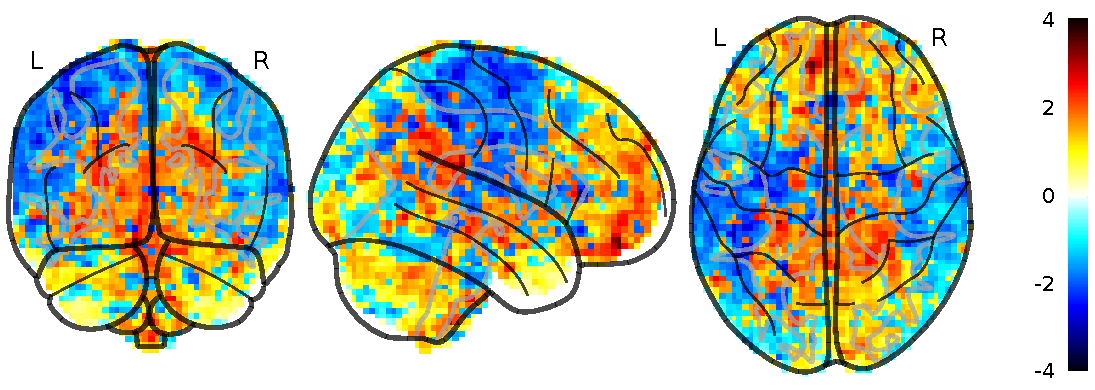
\includegraphics[width=\columnwidth]{figures/lepping_2017-399_original_brain.pdf} & 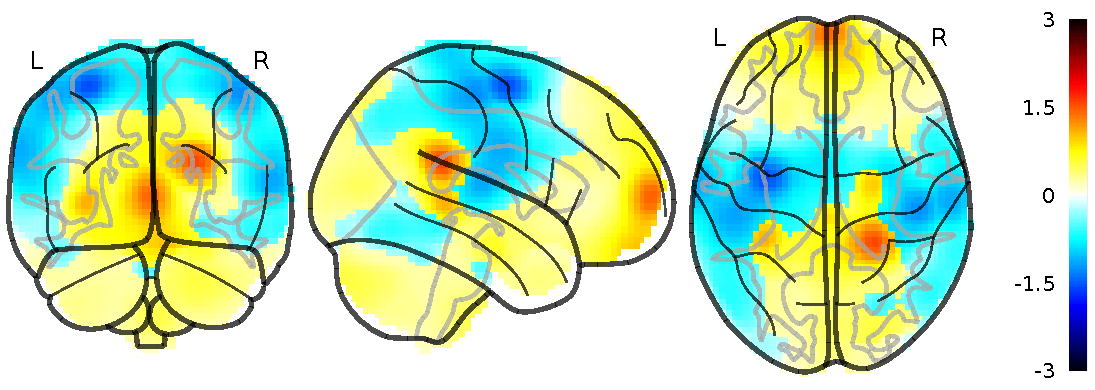
\includegraphics[width=\columnwidth]{figures/lepping_2017_trainval-399_ntfa_reconstruction.pdf} \\
        \textsf{\textbf{Reconstruction (HTFA)}} & \textsf{\textbf{Squared residuals (NeuralTFA)}} \\
        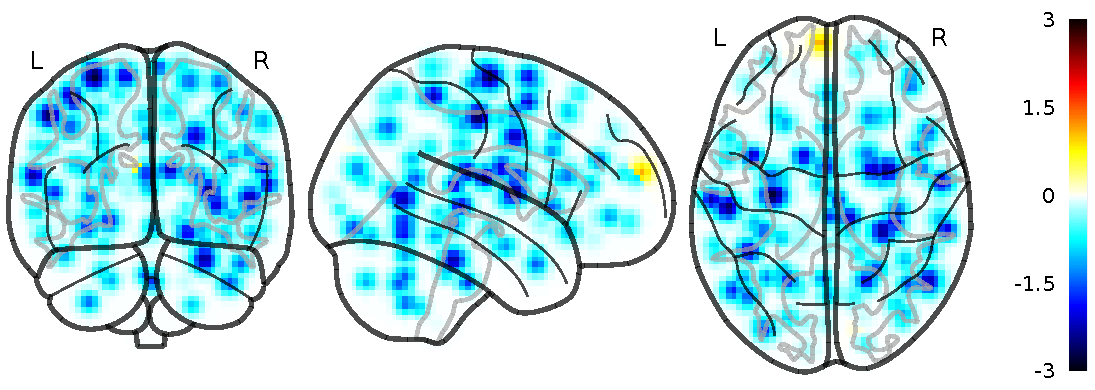
\includegraphics[width=\columnwidth]{figures/lepping_2017_trainval-399_htfa_reconstruction.pdf} &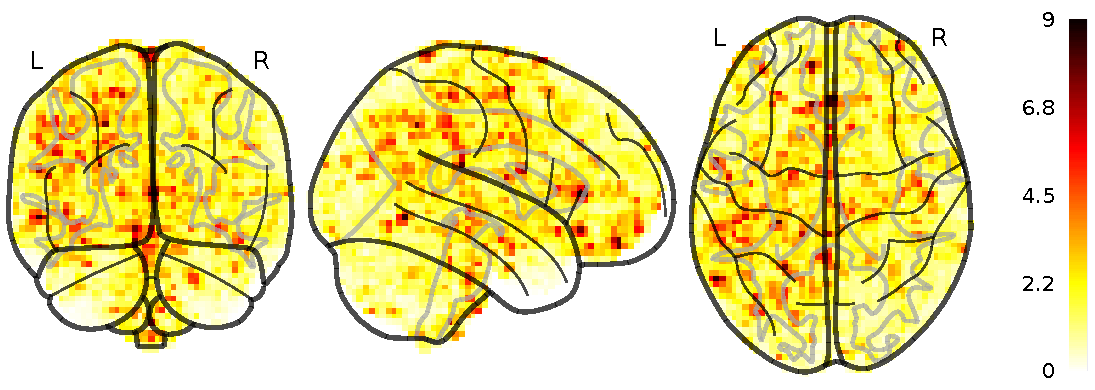
\includegraphics[width=\columnwidth]{figures/lepping_2017_trainval-399_ntfa_reconstruction_diff.pdf}
    \end{tabular}
    \caption{\textbf{Reconstructions for the Depression dataset}: The original image (top-left) enjoys a better reconstruction with $K=100$ by NTFA (top-right) than under HTFA (bottom-left).  NTFA's residuals (bottom-right) show that it captures detail across the brain rather than selectively reconstructing particular regions.}
    \label{fig:lepping-reconstruction}
    %\vspace{-1em}
\end{figure*}

The advantage of incorporating neural networks into the generative model is that it enables us to explicitly reason about multimodal response distributions and effects that vary between individual samples.  The network weights $\theta$ are shared across trials, as are the stimulus and participant embeddings $z^\scs_s$ and $z^\scp_p$. This allows NTFA to capture statistical regularities within a whole experiment.  At the same time, the use of neural networks ensures that differences in embeddings can be mapped onto a wide range of spatial and temporal responses.  Whereas the hierarchical Gaussian priors in HTFA implicitly assume that response distributions are unimodal and uncorrelated across different factors $k$, the neural network in NTFA is able to model such correlations by jointly predicting all $K$ factors.

While neural network models can have thousands or even millions of parameters, we emphasize that  NTFA in fact has a \emph{lower} number of trainable parameters than HTFA.  TFA and HTFA assume fully-factorized variational distributions, requiring $O(NK+NTK)$ learned parameters for $N$ trials with $T$ time points. In NTFA, the networks $\eta^\scf$ and $\eta^\scw$ will have $O(D(D+K))$ parameters each, whereas the variational distribution will have $O(D(P+S)+PK+NTK)$ parameters.

In practice, scanning time limitations impose a trade-off between $N$ and $T$ (the number of trials in a scanning run, and the length of a trial). For this reason $NTK$ does not always dominate $NK$, since often $T\propto O(10)$.  We can then choose $D\propto O(1)$ and $K \propto O(100)$, and if we label constant factors $c$, the total number of parameters becomes $O(cD^2 + cDK)$, making $O(cDK)$ the dominant term.  NTFA can have orders of magnitude fewer parameters when $D=2$ as compared to HTFA.

\vspace{-1.0em}
\section{Experiments}
\vspace{-1em}
\label{sec:experiments}

\subsection{Datasets}
\vspace{-1em}
\label{subsec:datasets}

We evaluate NTFA on four datasets. First, we verify that NTFA can recover a ground-truth embedding structure that, by construction, contains clearly distinguishable participant and stimulus clusters.

We present analysis of a previously unpublished in-house dataset, a pilot study pertaining to the subjective experience of fear.  We present embedding results from these datasets analyzed without their resting-state trials.  These experimental datasets vary in several qualities including the number of participants, time points, and voxels, and also task variables, testing how NTFA performs in a variety of experimental contexts.

Finally, we verify that NTFA can reconstruct the publicly available ``Pie Man'' dataset used to evaluate previous fMRI analysis models \citep{Anderson2016}. We consider a second publicly available dataset on emotional sounds and music, which contains many stimulus and participant categories \citep{10.1371/journal.pone.0156859}.

\textbf{Synthetic Data}: %To demonstrate that in addition to accurate reconstructions NTFA can also learn meaningful embeddings, 
We consider a simulated dataset in which there are three participant groups of five participants each, which we call \emph{Group 1}, \emph{Group 2} and \emph{Group 3}. All participants underwent two categories of hypothetical stimuli, called \emph{Baseline} and \emph{Task}, with five stimuli within each category.  Each participant underwent a single hypothetical scanning run with rest trials interleaved between stimuli. We manually defined three distinct factors in a standard MNI\_152\_8mm brain. We then sampled participant embeddings $\{z_1^\scp,...,z_{15}^\scp \}$ and stimulus embeddings $\{ z_1^\scs,...,z_{10}^\scs\}$, from mixtures of three and two distinct Gaussians respectively. We set the means for these Gaussians to meet the following conditions under noisy combination:

\begin{itemize}[labelwidth=0.5em, 
                labelsep=0.5em, 
                leftmargin=1.0em,
                topsep=0em,
                label={\tiny\raisebox{0.7ex}{\textbullet}}]
% \vspace{-1em}
    \item All participants show no whole-brain response during rest besides random noise.
    \item Under \emph{Baseline} stimuli, Group 1 exhibits half the response in the first region as compared to under \emph{Task} stimuli, on average.  The rest of the brain shows no response. Similarly, Group 2 and Group 3 exhibits a response in the second and third regions respectively, while the rest of the brain shows no response.
    \item Each \emph{Baseline}/\emph{Task} stimulus provokes a response lower or higher than the stimulus category's average based on the stimulus embedding's location.
% \vspace{-1em}
\end{itemize}

\textbf{The Fear and Affective Videos (``AffVids'')}: This is a dataset for a pilot study that we have carried out in-house. A total of 22 participants watched videos depicting fear-related content and rated affective and emotional impact after each clip. The stimuli consisted of 36 videos, separated into three fear-related content situations (spiders, heights, and social situations), each clip lasting 20 seconds. Participants provided subjective experience ratings (e.g.~how much fear they felt) after each clip. The fMRI data contained 81,638 voxels and 1656 time points per scanning run.

\textbf{Emotional Musical and Nonmusical Stimuli in Depression (``Depression'')}
\citep{10.1371/journal.pone.0156859}\footnote{This data was obtained from the OpenfMRI database. Its accession number is ds000171.}: 19 participants with major depressive disorder, and 20 control participants (N=39) underwent emotional musical and nonmusical stimuli to examine how neural processing of emotionally provocative auditory stimuli is altered within the anterior cingulate cortex and striatum in depression.  The fMRI data had 353,600 voxels, and 105 time points for each scanning run.  We refer to this dataset by the shorthand \emph{Depression}, and show an example reconstruction from it in Figure \ref{fig:lepping-reconstruction}.

\textbf{Pie Man Narrative Listening (``Pie Man'')} \citep{simony2016dynamic}\footnote{\scriptsize \url{http://arks.princeton.edu/ark:/88435/dsp015d86p269k}}: In a between-subjects design, participants were assigned to one of four experimental stimulus categories that varied in the amount of structured narrative content that was presented. Participants either listened to an intact audio recording of the story \emph{Pie Man} (N = 36), or the same recording with paragraphs scrambled (N = 18) or with words scrambled (N = 25). A fourth group of participants were not presented with any recordings (N = 36). The fMRI data had 61,367 voxels and 300 time points for each scanning run. The narrative was presented at a story-telling event organized by \emph{The Moth}.

\vspace{-1em}
\subsection{Training and Test Sets}
\label{subsec:train_val_sets}
\vspace{-1em}

We have split our datasets into training and test sets in a manner that ensures that the training set always contains at least one trial for each participant $p \in \{1,\ldots,P\}$ and each stimulus $s \in \{1,\ldots,S\}$.  To do so, we construct a matrix of $(p,s) \in \{1,\ldots,P\}\times \{1,\ldots,S\}$ with participants as rows and stimuli as columns, choose its modulo-columns diagonals ($\{(p, s) : p \bmod S = s \}$) as validation pairs.  All blocks with these pairs of participant and stimulus belong to the test set; all others belong to the training set.

When maximizing the IWAE bound on the log evidence over the training set, we update all parameters $\theta$ and $\lambda$.  For our test set, we ran inference separately, adjusting only the single-trial (local) variational parameters $\lambda^\scw_{n,t}$ for the trials $n$ and time-points $t$ having $p_n$ and $s_n$ such that $p_n \bmod S = s_n$.  We update nothing else during inference on the test set.

The Pie Man experiment exposed many participants to only one stimulus, so we were unable to separate it into a training and test set.  The other two real datasets provide data for each $(p, s)$ of participant and stimulus, and for these all results come from the test set.
\vspace{-1em}
\subsection{Model Architecture and Training}
\label{subsec:model_architecture}
\vspace{-1em}
We here describe the model architectures employed in NeuralTFA.  In general, for the experiments on real datasets in this paper we set $D=2$ and $K=100$ arbitrarily.  For the synthetic dataset, we treated $K=3$ as a known ground-truth.  We report the number of parameters in our model, and in HTFA, in Table \ref{table:parameter_counts}.
We define $\eta^\scf_\theta(\cdot)$ as an input layer, hidden layer, and output layer with PReLU activations $f$.
\begin{align}
    f(x) &= \max (0, x) + a \min (0, x) \\
    \eta^\scf_\theta &\equiv \mathbb{R}^{8K \times 4D} \circ f \circ \mathbb{R}^{4D \times 2D} \circ f \circ \mathbb{R}^{2D \times D} \\
     \eta^\scf_\theta(z^\scp) &: \mathbb{R}^D \mapsto \mathbb{R}^{8K}
\end{align}
The matrices specifying the linear transformations are given in the neural network weights $\theta$, and we extract the factor parameters $\scf, x$ and $\scf, \rho$ from the appropriate dimensions of the $8K$-dimensional result.  We define the network $\eta^\scw_\theta(\cdot)$ generating factor weights similarly, though operating over both embeddings.

\begin{align}
    \eta^\scw_\theta &\equiv \mathbb{R}^{2K \times 8D} \circ f \circ \mathbb{R}^{8D \times 4D} \circ f \circ \mathbb{R}^{4D \times 2D} \\
        \eta^\scw_\theta \left( z^\scp, z^\scs \right) &: \mathbb{R}^{2D} \mapsto \mathbb{R}^{2K}
\end{align}

\begin{figure}[!t]
    \centering
    \textsf{\textbf{Ground truth}} \\
    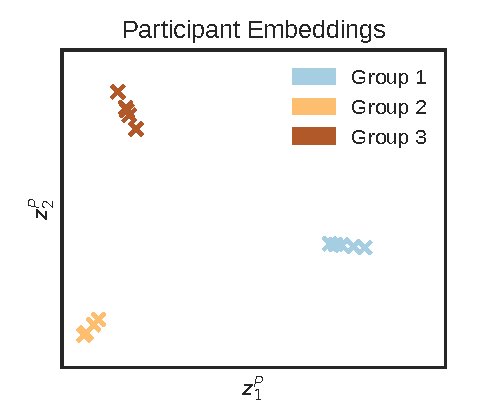
\includegraphics[width=0.45\columnwidth]{figures/participant_embedding_means_true_notick.pdf}
    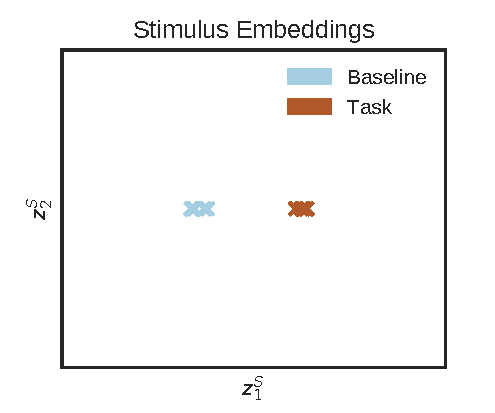
\includegraphics[width=0.45\columnwidth]{figures/stimuli_embedding_means_true_notick.pdf} \\
    \textsf{\textbf{Inferred}} \\
    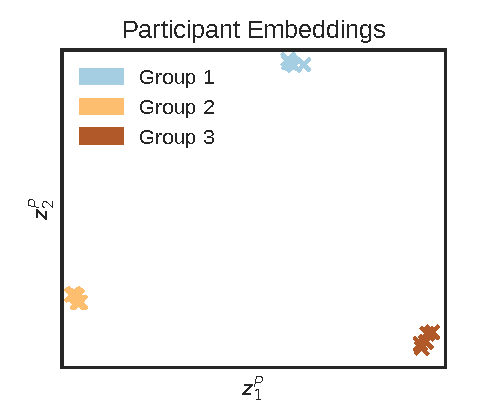
\includegraphics[width=0.45\columnwidth]{figures/participant_embedding_means_notick.pdf}
    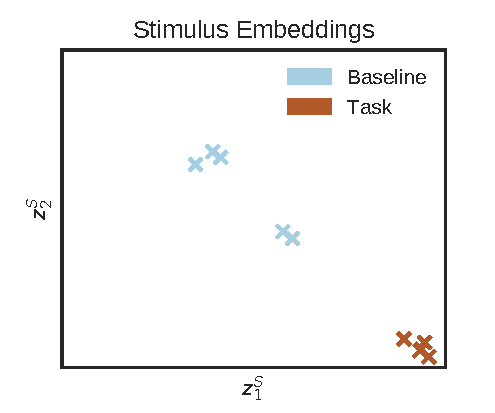
\includegraphics[width=0.45\columnwidth]{figures/stimuli_embedding_means_notick.pdf}
    \caption{\textbf{Inferred embeddings for synthetic data}: We apply NTFA to a dataset in which three groups of participants exhibit varying levels of response in three different brain regions to \emph{Task} and \emph{Baseline} simuli. Without prior knowledge of participant groups and stimulus categories, NTFA recovers these conditions as participant and stimulus embeddings. Only the relative spatial arrangement is of interest.}
    \label{fig:synthetic_embeddings}
    %\vspace{-1.5em}
\end{figure}

\begin{table}[!t]
\caption{\textbf{Parameter counts}: When using low-dimensional embeddings, NTFA has roughly as many parameters as HTFA for the Pie Man dataset, and orders of magnitude fewer learnable parameters for other datasets, which have many more trials than participants ($N \gg P$).  We chose $K=100$ for both models across the real datasets, and $D=2$ for NTFA.}
\label{table:parameter_counts}
% \vspace{-1.0em}
%\vskip 0.15in
\begin{center}
\begin{tabular}{lcc}
\toprule
\textbf{Dataset} & \textbf{HTFA} & \textbf{NTFA} \\
 & \textbf{parameters} & \textbf{parameters} \\
\midrule
Pie Man  & $1.02\times 10^7$ & $1.02\times 10^7$ \\
Depression & $2.53\times 10^7$  & $2.61 \times 10^6$ \\
AffVids & $1.64\times10^8$ & $8.88\times 10^6$ \\
Synthetic ($K=3$) & $2.16\times10^4$ & $1.90\times10^4$ \\
\bottomrule
\end{tabular}
\end{center}
%\vspace{-0.75em}
% \vspace{-1.0em}
%\vspace{-15pt}
\end{table}
\begin{table}[!t]
% \vspace{-1.0em}
\caption{\textbf{Model performance} in terms of log likelihood and and log evidence. We approximate the log evidence with an importance-weighted estimator \citep{Burda2016}. For all datasets except Pie Man, we evaluate on a test set of held out subject-stimuli pairs. This is not possible for the Pie Man data, for which we report training set performance.}
\label{table:reconstruction_errors}
% \vspace{-1.0em}
%\vskip 0.15in
\begin{center}
\begin{tabular}{lcc}
\toprule
 & \textbf{HTFA} & \textbf{NTFA} \\
\midrule
\multicolumn{3}{l}{\textbf{Log likelihood (Reconstruction Loss)}}\\
~Synthetic ($K\!=\!3$) & $-4.69 \times 10^6$ & $\mathbf{-4.68 \times 10^6}$ \\
~AffVids & $-1.59 \times 10^8$ & $\mathbf{-1.56 \times 10^8}$ \\
~Depression & $-1.69 \times 10^8$ &  $\mathbf{-1.48 \times 10^8}$\\
~Pie Man*  &  $-5.01 \times 10^9$ & $\mathbf{-4.36 \times 10^9}$ \\
\midrule
\multicolumn{3}{l}{\textbf{Log marginal likelihood (IWAE bound)}}\\
~Synthetic ($K=3$) & $-4.72 \times 10^6$ & $\mathbf{-4.68 \times 10^6}$ \\
~AffVids & $-1.61 \times 10^8$ & $\mathbf{-1.56 \times 10^8}$ \\
~Depression & $-1.71 \times 10^8$ &  $\mathbf{-1.49 \times 10^8}$\\
~Pie Man*  & $-5.24 \times 10^9$ & $\mathbf{-4.38 \times 10^9}$ \\
\bottomrule
\end{tabular}
\end{center}
%\vspace{-0.75em}
\vspace{-1em}
%\vspace{-15pt}
\end{table}
We performed optimization using the Adam algorithm \citep{Kingma2015}, for 1000 steps per dataset (including another 1000 on the local parameters of the test set), which was usually more than enough for the objective to converge.  We used learning rates of 0.01 for the variational parameters $\phi$ and 0.0001 for the generative parameters $\theta$.  We scheduled the learning rates with a patience of 100 epochs, and a multiplicative decline in learning rates (by 0.5 whenever learning rates were decreased), which was unnecessary for the real datasets.  We used $L=100$ particles to calculate the log likelihood and the IWAE evidence bound.
\vspace{-1em}
\subsection{Evaluation}
\label{subsec:evaluation}
\vspace{-1em}

We compare NTFA to HTFA in its reconstruction loss and the log marginal likelihood (a.k.a~the model evidence). We report the log-likelihood (a.k.a.~the reconstruction loss) and an importance-weighted lower bound to the log evidence for each dataset's test set (except for Pie Man).  We then examine the inferred embeddings for patterns based on stimulus categories, sorted participant categories, and invididual differences.
\begin{figure}[!t]
    % \vspace{-1em}
    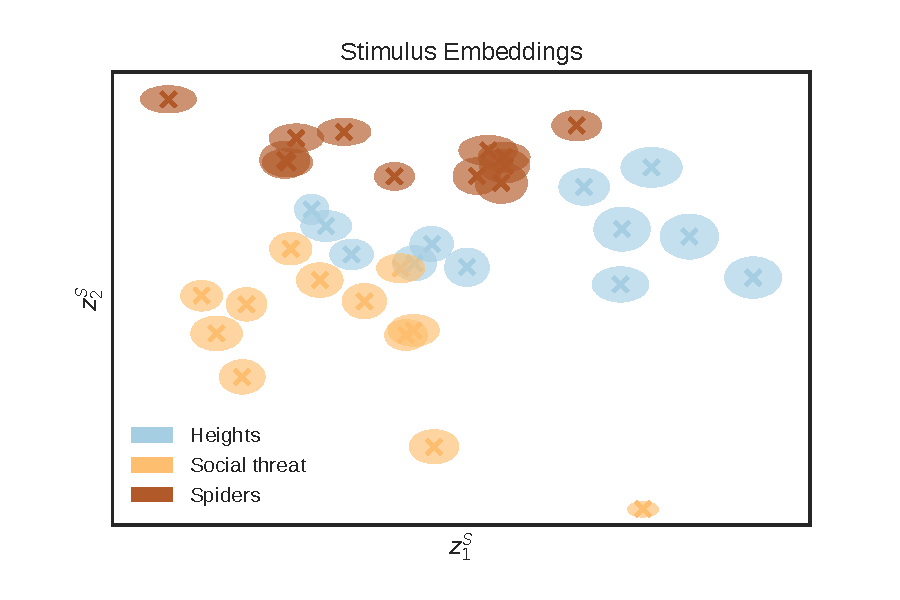
\includegraphics[width=\columnwidth]{figures/affvids_norest_task_embedding.pdf}
    % \vspace{-1.5em}
    \caption{Stimulus embeddings from the AffVids dataset. Crosses indicate the location of the (approximate) posterior mean, and ellipses display (approximate) posterior covariance. Stimulus embeddings recovered groups of fear stimuli corresponding to heights, spiders, and social threats.  The overlap may reflect intentionally low fear intensity on the part of the stimulus designers, leading to decreased separability.}
    \label{fig:affvids-task-embeddings}
    \vspace{-1em}
\end{figure}
Across datasets, NTFA exhibits a higher log-likelihood than the state-of-the-art model HTFA (Table \ref{table:reconstruction_errors}), with the same number ($K=100$) of latent factors.  Since our Synthetic dataset consisted of images generated solely from a limited number of factors and white noise, it offered the least performance gain in moving from HTFA to NTFA.  In contrast, NTFA enjoys its greatest performance improvements in datasets like AffVids, in which the sharing of embeddings allows us to learn fine-grained individual stimulus representations while also reconstructing noisy data.  We visualize an example reconstruction from the Depression dataset, on which NTFA also enjoyed substantial performance improvements over HTFA, in Figure \ref{fig:lepping-reconstruction}.

\textbf{Synthetic Data}: For synthetic data, NTFA recovers stimulus and participant embeddings that are qualitatively very similar to the embeddings that we used to generate the data (Figure \ref{fig:synthetic_embeddings}). We emphasize that embeddings are learned directly from the synthetic data in an entirely unsupervised manner, which means that there is in principle no reason that we would expect embeddings to be exactly the same. However, we do observe that learned embeddings for participants and stimuli are well-separated, appear to have some variance, and are invariant under linear transformations. Moreover, given the ``true'' number of factors ($K=3$), NTFA reconstructs synthetic data better than HTFA.

\textbf{Fear and Affective Videos dataset}: On the AffVids dataset, NTFA achieves better reconstructions than HTFA, as reported in Table \ref{table:reconstruction_errors}.  In an analysis without resting-state data, NTFA uncovered stimulus embeddings that clustered by category (Figure \ref{fig:affvids-task-embeddings}).  The participant embeddings uncovered three groups: the more frightened, the less frightened, and those sensitive to particular fears (Figure \ref{fig:affvids-subject-embeddings}). Participant embeddings for individual fear categories are shown in Figure \ref{fig:affvids-subject-embeddings}. Participants were not recruited in specific groups (e.g.~arachnophobes and acrophobes), and stimuli could be categorized multiple ways (e.g.~by kind or degree).  We observe that most participants carried a greater fear of heights (left) and social threat (right) than of spiders (middle).  A scattering of individuals in the mid-left of the embedding space appeared to suffer little overall fear in any stimulus category, while those further out from the centroid had more varied fear experiences across categories.  Few individuals showed high mean fear ratings across stimulus categories.

\begin{figure}[!t]
    % \vspace{-1em}
    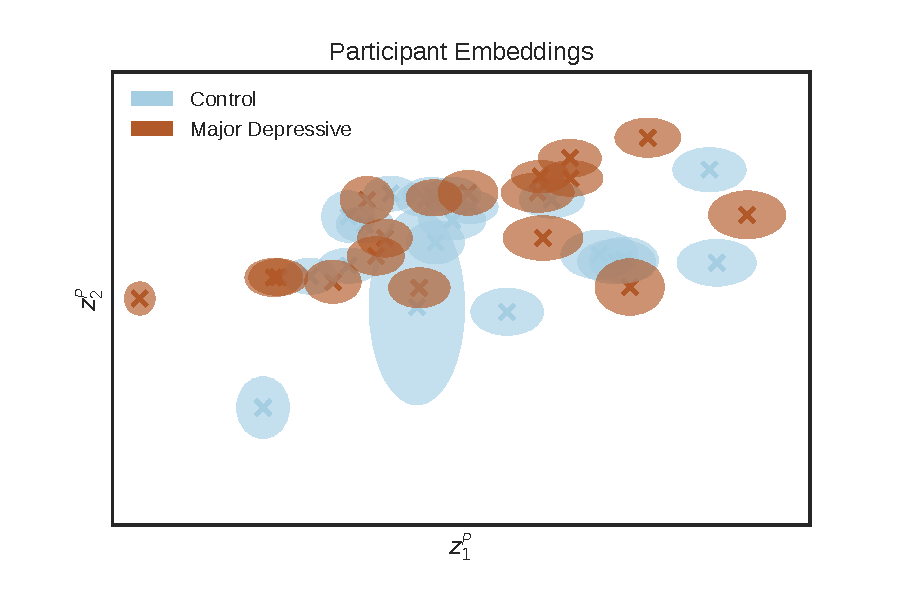
\includegraphics[width=\columnwidth]{figures/lepping_2017_noresponse-subject_embedding.pdf}
    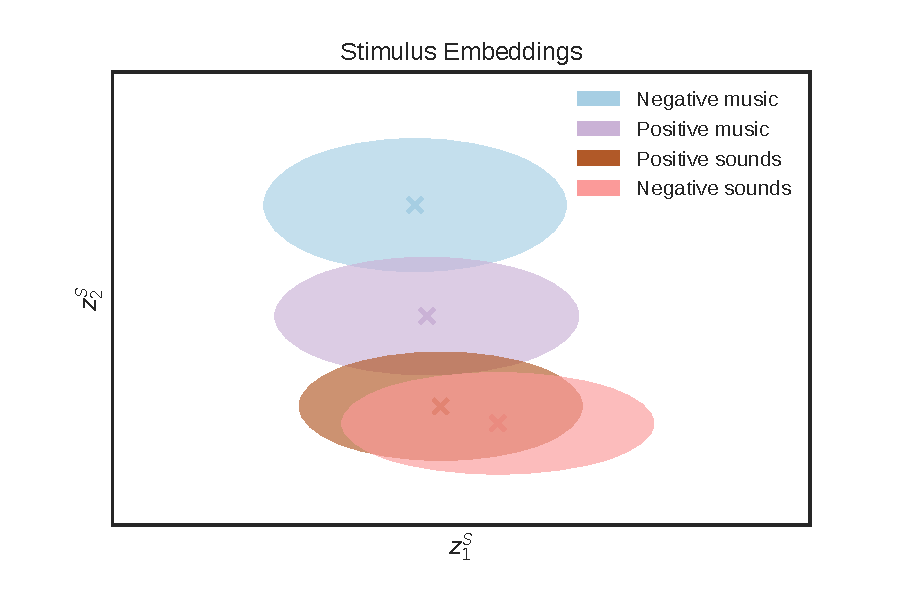
\includegraphics[width=\columnwidth]{figures/lepping_2017_noresponse-task_embedding.pdf}
    % \vspace{-1.5em}
    \caption{Participant and stimulus embeddings from the Depression dataset \citep{10.1371/journal.pone.0156859}.  Crosses indicate the location of the (approximate) posterior mean, and ellipses display (approximate) posterior covariance. \textbf{Above}: Participant embeddings spanned from mostly depressed (lower-left) to mostly control (upper-right) \textbf{Below}: Stimulus embeddings varied from tonal (top-left) to atonal (bottom-right).}
    \label{fig:lepping-embeddings}
    \vspace{-1.5em}
\end{figure}

\begin{figure*}[!h]
    % \vspace{-1em}
    \centering
    \textsf{Participant Embeddings} \\
    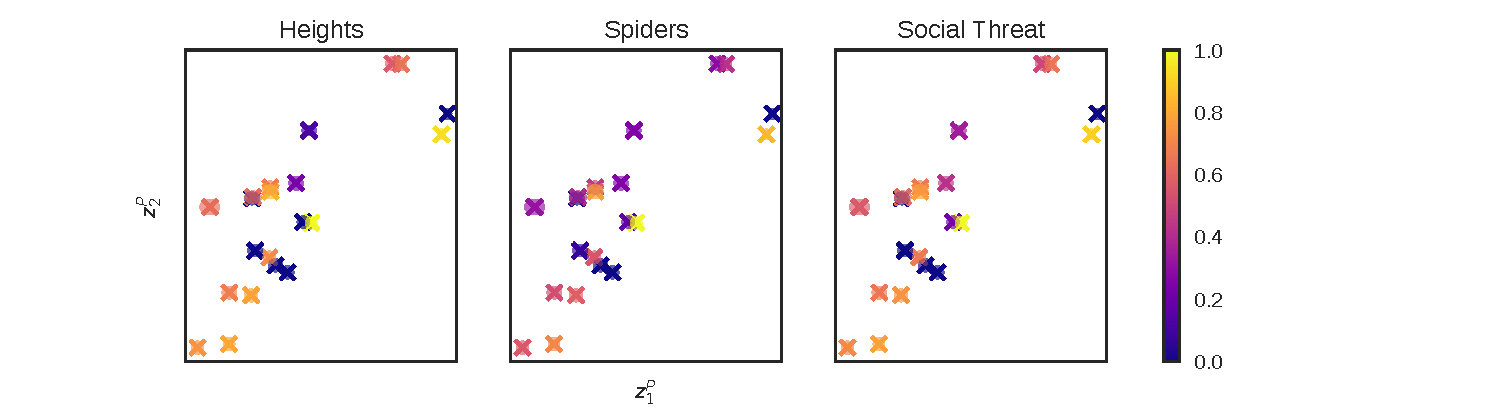
\includegraphics[width=\textwidth]{figures/affvids_norest_subject_heatmap.pdf}
    % \vspace{-1.5em}
    \caption{Participant embeddings from the AffVids dataset, color-coded three times by their reported level of fear across the stimulus categories of heights, spiders, and social threats. Cooler colors indicate lower mean fear ratings within a stimulus category, while warmer colors indicate higher mean fear ratings.  Crosses indicate the location of the (approximate) posterior mean, and ellipses display (approximate) posterior covariance.}
    \label{fig:affvids-subject-embeddings}
    % \vspace{-1em}
\end{figure*}

\textbf{Emotional Musical and Nonmusical Stimuli in Depression dataset}: On this dataset, NTFA similarly achieved better reconstruction loss than HTFA.  The supplied metadata labeled stimuli by category rather than individually, so stimulus embeddings only acquired a linear gradation from tonal/musical to atonal/nonmusical.  Participant embeddings for major depressive and control-group participants were closely scattered around a semi-apparent dividing line (Figure \ref{fig:lepping-embeddings}).  Regularization could potentially separate the groups.  We only labelled the embeddings for visualization; NTFA discovers this structure unsupervised.

\textbf{The ``Pie Man'' Narrative Listening dataset}: The Pie Man dataset \citep{simony2016dynamic} has previously been used to evaluate TFA and HTFA  \citep{manning2018probabilistic}.  Each participant underwent one trial with one stimulus in each scanning run, so only stimulus embeddings were shared across trials.  NTFA did manage to improve over HTFA's reconstruction loss on this dataset, but it failed to disentangle meaningfully varied embeddings.  We do not show its embedding plots.

\vspace{-1em}
\section{Discussion}
\vspace{-1em}

We have introduced Neural Topographic Factor Analysis (NTFA), an unsupervised model of spatio-temporal fMRI data which learns low-dimensional embeddings for participants and stimuli.  We demonstrated that NTFA can recover ground-truth embedding clusters in synthetically generated data, and that it can reconstruct three datasets of real fMRI data better than the state-of-the-art using as few hidden factors as $K=100$.  NTFA attains higher log-likelihood than HTFA across data sets, for the same number of latent factors. When we set $D=2$, NTFA learned embeddings from the real fMRI datasets that appeared to vary in a neuroscientifically meaningful way.  This suggests that NTFA captures meaningful aspects of the underlying data.

Contrary to expectations of how a model can achieve superior reconstruction, NTFA requires fewer parameters.  For the AffVids dataset, NTFA required on the order of 8.88 million parameters, as opposed to HTFA's 164 million parameters, two orders of magnitude of advantage in compressing and representing large datasets.  We see this advantage in datasets with many more trials than participants ($N \gg P$), as shown in Table \ref{table:parameter_counts}.

NTFA provides a path towards a more data-driven, discovery-oriented approach to investigating when neural activity varies across participants and stimuli, and when it remains relatively similar.  In future work, we will follow up on these findings by exploring how various hyperparameters affect sensitivity to such relationships.

% NTFA's performance on high-dimensional spatio-temporal data with comparatively few parameters demonstrates the utility of combining deep generative models with embeddings for variations across trials that are known to the modeler.  When considering data in which variations are not necessarily Gaussian around a spatial template, NTFA shows its greatest improvements over HTFA by learning the functional form of these variations.

On all but one of the applicable datasets, NTFA revealed apparent separation between stimuli and/or participant embeddings. This suggests that it can leverage factor analysis techniques to inform high-level reasoning and hypothesis testing about the relationship between participants and experimental stimuli.
%One of the datasets (AffVids) produced promising reconstruction results although less interpretable embedding results. This is suggestive of the NTFA procedure is capturing meaningful aspects of the underlying data, but not revealing a higher order relationship between stimuli or participants. Future work will be able to follow up on these initial findings by exploring how various parameter choices might improve sensitivity to such relationships. That is, it is possible that increasing the dimensionality of the embeddings to more than two might reveal more complex relationships across stimuli and participants.

Neuroscientifically, the question remains open how efficiently factor analysis models such as TFA, HTFA, and NTFA actually compress data.  The brain works on a many-to-many mapping from neural dynamics to observable psychological phenomena, with degeneracy at every level \citep{Edelman2001,Marder2011}.  Future studies of such methods could usefully consider how the reconstruction loss declines as a function of the number of latent factors $K$.  We arbitrarily fixed $K=100$, while studies such as \cite{manning2018probabilistic} found optimal values as high as $K=700$ through cross-validation.  Do such increases in parameterization lead to overfitting of fixed datasets, or can increasing NTFA's model capacity lead to successful generalization on spatio-temporal neuroimaging data?%  A transfer learning study would elucidate the question.

Practically, these techniques reflect a growing and urgent need for scalable analysis approaches in the neuroscience community. There are international efforts to collect fMRI datasets of hundreds or thousands of participants performing numerous cognitive tasks. Traditional analyses which do not efficiently compress the underlying data are not suited to guide inferences performed across such large samples. The approach we describe here is ideally suited for such datasets and offer the prospect of capturing meaningful, interpretable aspects of the data for both clinicians and researchers.

% \vspace{-1em}
% \subsubsection*{Acknowledgments}

% The authors thank Jeremy Manning for insightful conversations during his visit.  This work was supported by Intel, startup funds from Northeastern University, the National Science Foundation (NCS 1835309), and the US Army Research Institute for the Behavioral and Social Sciences (ARI W911NF-16-1-0191).

\bibliography{aistats_ntfa}
\bibliographystyle{plainnat}

\end{document}
